\subsection{Топологии нейронных сетей}

Структура нейронных сетей тесно связана с используемыми алгоритмами обучения.
В общем случае можно выделить три фундаментальных архитектуры нейронных сетей.

\subsubsection{Однослойные прямого распространения}

В многослойных нейронной сети нейроны располагаются по слоям.
В простейшем случае у такой сети существует входной слой узлов источника, информация от которого передается на выходной слой нейронов (вычислительные узлы), но не наоборот. 
Такая сеть называется сетью прямого распространения или ациклической сетью.
\begin{figure}[h]
\center{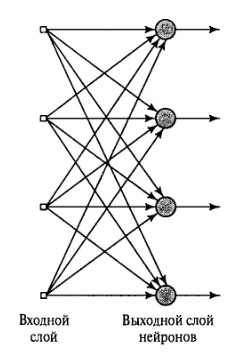
\includegraphics[width=0.4\linewidth]{OneLayer.png}}
\caption{Однослойная сеть прямого распространения}
\label{ris:OneLayer}
\end{figure}

На рис.~\ref{ris:OneLayer} показана структура такой сети для случая четырёх узлов в каждом из слоев (входном и выходном).
Такая нейронная сеть называется однослойной, при этом под единственным слоем подразумевается слой вычислительных элементов (нейронов).
При подсчёте числа слоев мы не принимаем во внимание узлы источника, так как они не выполняют никаких вычислений.\cite{NejronnyeSeti}

\subsubsection{Многослойные прямого распространения}

Другой класс нейронных сетей прямого распространения  характеризуется наличием одного или нескольких скрытых слоев, узлы которых называют скрытыми нейронами или скрытыми элементами.
Функция последних заключается в посредничестве между внешним входным сигналом и выходом нейронной сети.
Добавляя один или несколько нейронных слоев мы можем выделить статистики более высокого порядка.
Такая сеть позволяет выделять глобальные свойства данных с помощью локальных соединений за счёт наличия дополнительных синаптических связей  и повышения уровня взаимодействий нейронов.
Способность скрытых нейронов выделять статистические зависимости высокого порядка особенно существенна, когда размер входного слоя достаточно велик.

Узлы источника входного слоя сети формируют соответствующие элементы шаблона активации (входной  вектор), которые составляют входной сигнал, поступающий на нейроны (вычислительные элементы) второго слоя (т.е. первого скрытого слоя).
Выходные сигналы второго слоя используются в качестве входных для третьего слоя и т.д.
Обычно нейроны каждого из слоев сети используют в качестве входных сигналов только выходные сигналы нейронов предыдущего слоя.
Набор выходных сигналов нейронов последнего слоя сети определяет общий отклик сети на данный входной образ, сформированный узлами источника входного слоя.

\begin{figure}[h]
\center{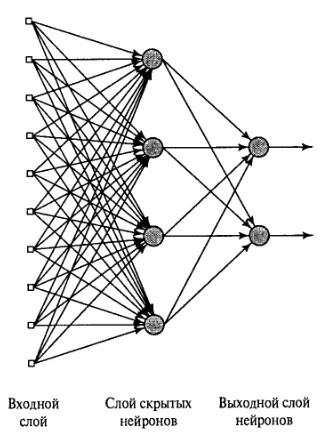
\includegraphics[width=0.4\linewidth]{ManyLayer.png}}
\caption{Многослойная сеть прямого распространения}
\label{ris:ManyLayer}
\end{figure}

Сеть, показанная на рис.~\ref{ris:ManyLayer}, называется сетью 10-4-2, так как имеет 10 входных, 4 скрытых и 2 выходных нейрона.
Нейронная сеть, показанная на рис.~\ref{ris:ManyLayer}, считается полносвязной в том смысле, что все узлы каждого конкретного слоя соединены со всеми узлами смежных слоев.
Если некоторые из синаптических связей отсутствуют, то такая сеть называется неполносвязной.\cite{NejronnyeSeti}

\subsubsection{Рекуррентные}
Рекуррентная нейронная сеть отличается от сетей прямого распространения наличием по крайней мере одной обратной связи.
Например, рекуррентная сеть может состоять из единственного слоя нейронов, каждый из которых направляет выходной сигнал на входы всех остальных нейронов сети.

\begin{figure}[h]
\center{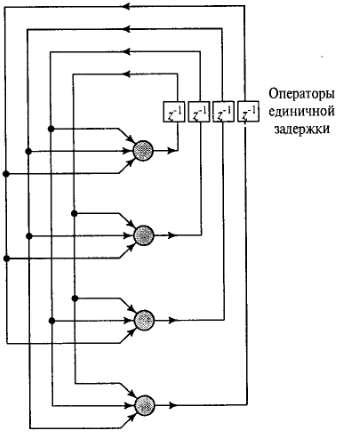
\includegraphics[width=0.4\linewidth]{Recurrent.png}}
\caption{Рекуррентная сеть без скрытых нейронных слоев}
\label{ris:Recurrent}
\end{figure}

Архитектура нейронной сети показана на рис.~\ref{ris:Recurrent}.
Стоит обратить внимание, что в нейронной сети нет обратной связи нейронов самих с собой.
Рекуррентная сеть, показанная на рис.~\ref{ris:Recurrent}, не имеет скрытых нейронов.
Наличие обратных связей в нейронных сетях оказывает непосредственное влияние на способность таких сетей к обучению и на их производительность.
Более того, обратная связь подразумевает наличие элементов единичной задержки, что приводит к нелинейному динамическому поведению.\cite{NejronnyeSeti}